\begin{frame}{How We Usually Predict Progress}
\begin{columns}[c]
\column{0.34\textwidth}
\centering
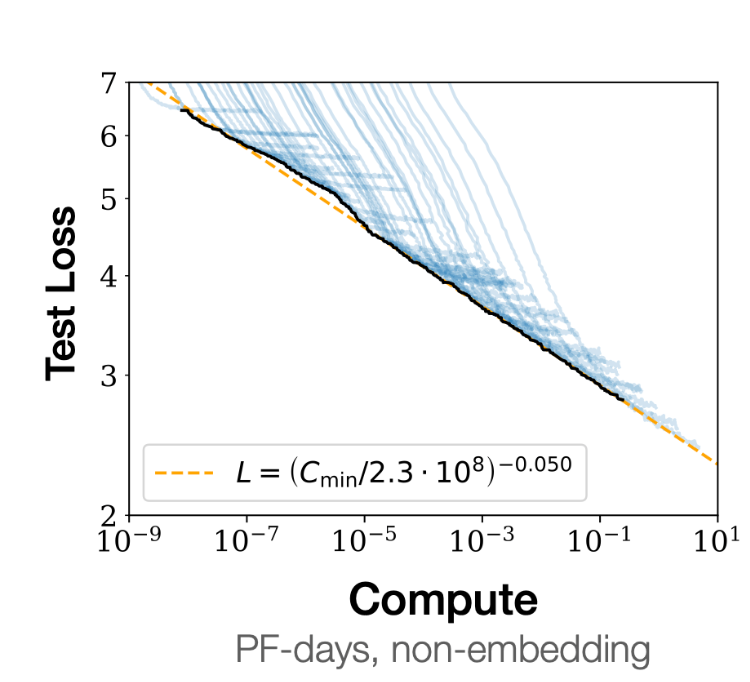
\includegraphics[width=\linewidth]{kaplan_compute}
\column{0.64\textwidth}
\centering
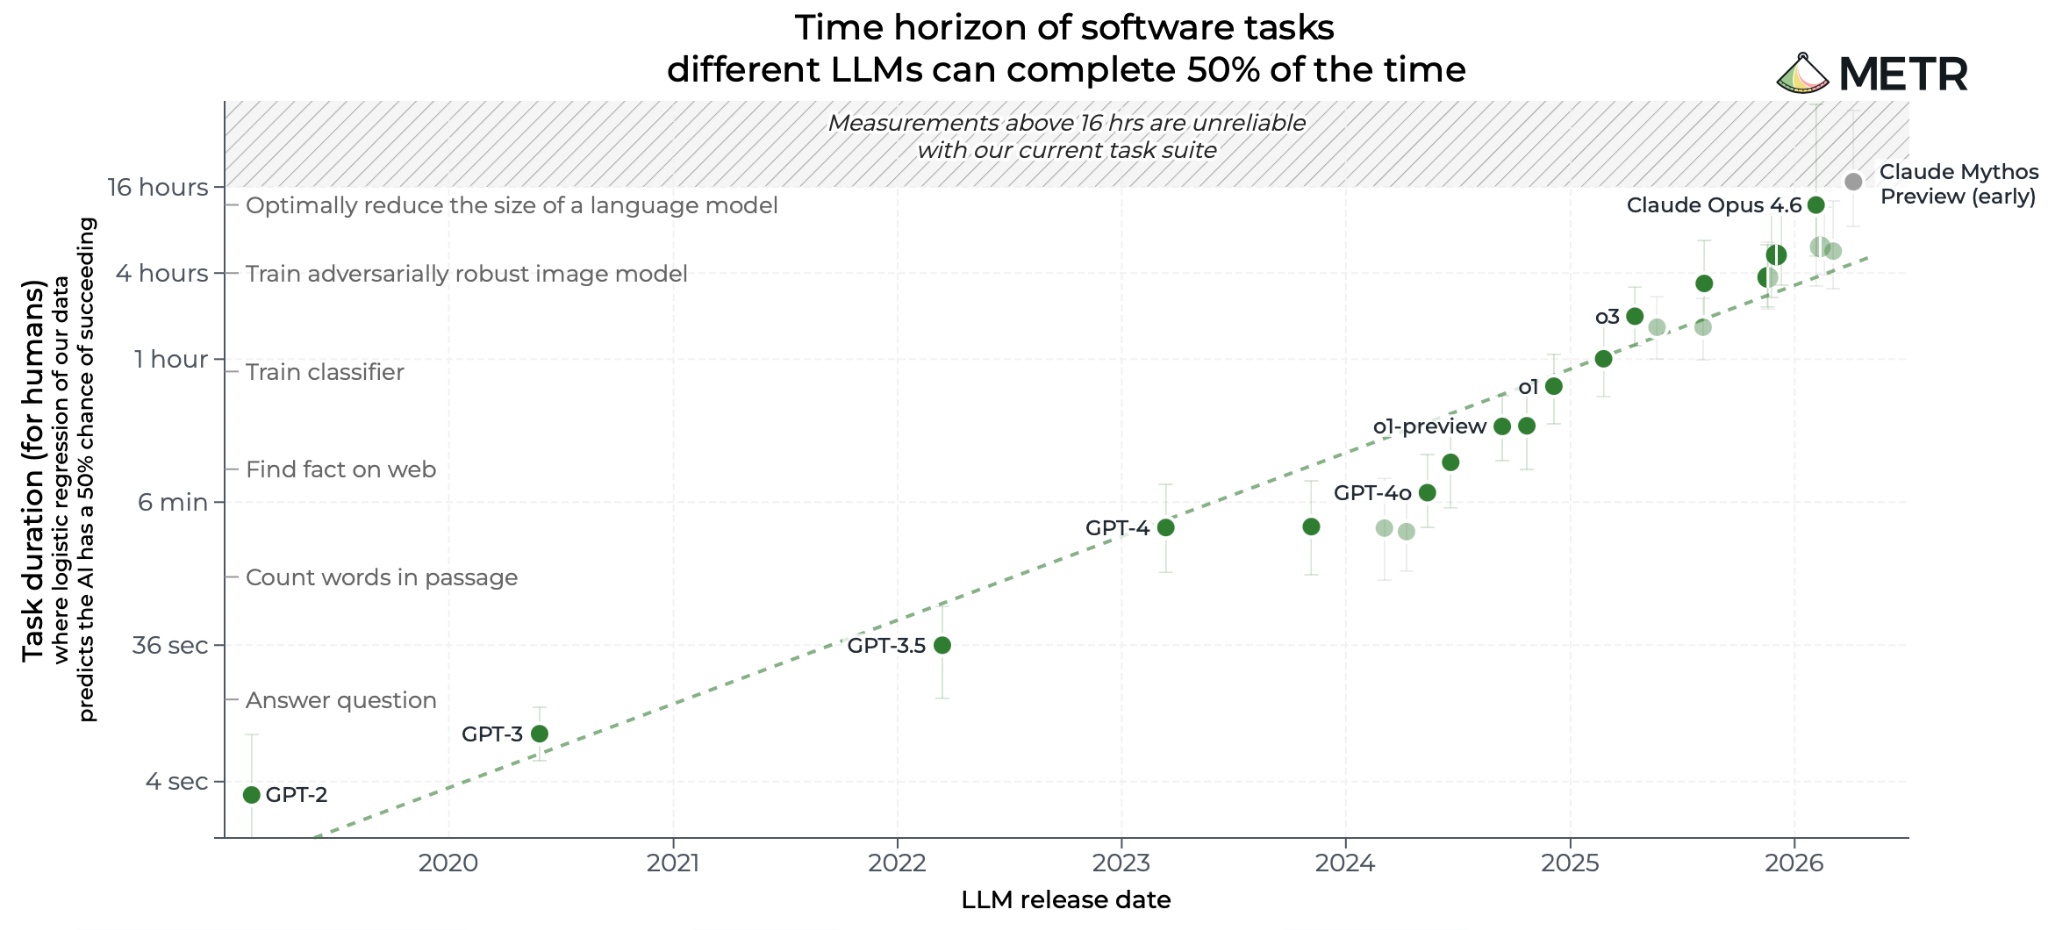
\includegraphics[width=\linewidth]{metr_time_horizon}
\end{columns}
\source{kaplan2020,kwa2025}
\end{frame}

\begin{frame}{Timelines Have Collapsed}
\centering
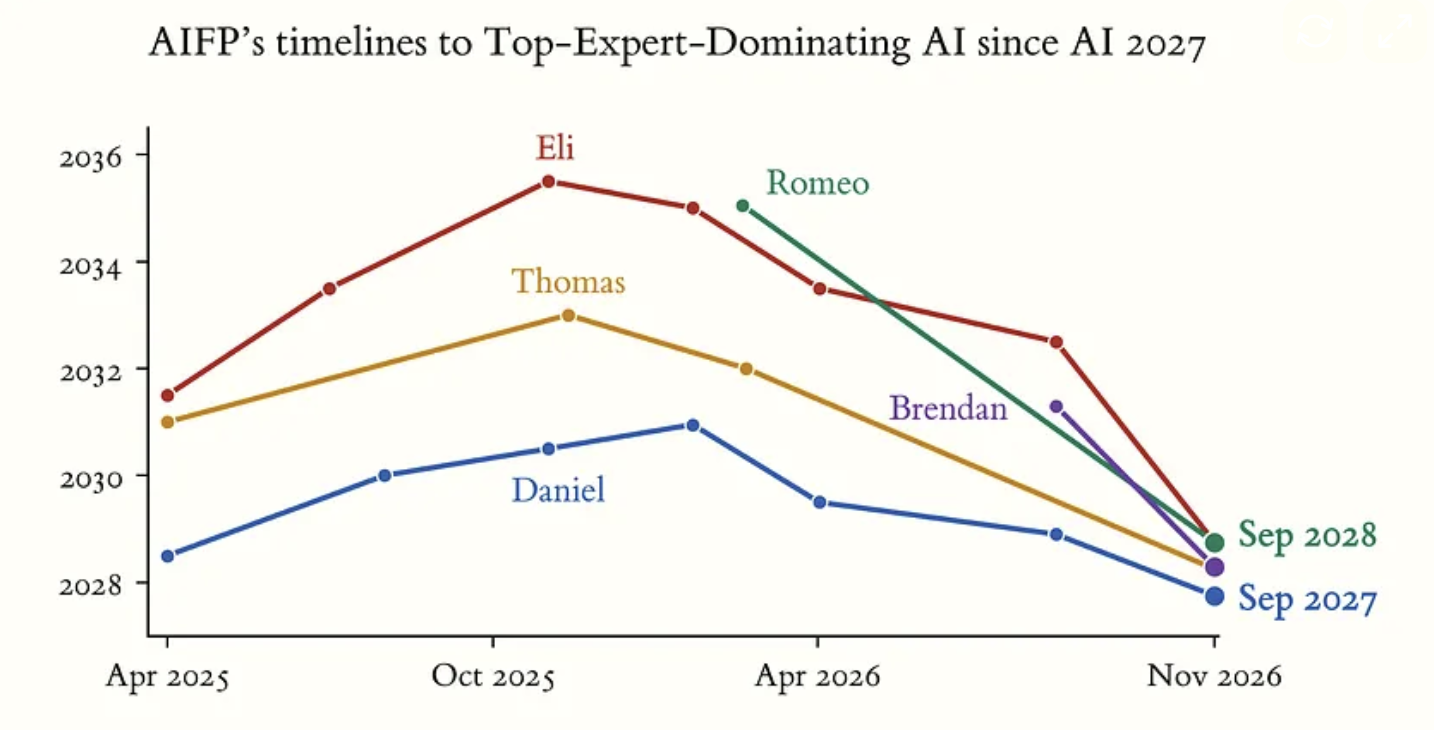
\includegraphics[height=0.72\textheight]{bib/lifland2026/figures/updates_of_timeliens}
\source{lifland2026}
\end{frame}

\begin{frame}{AI Might Take Over, and We Might All Die}
\centering
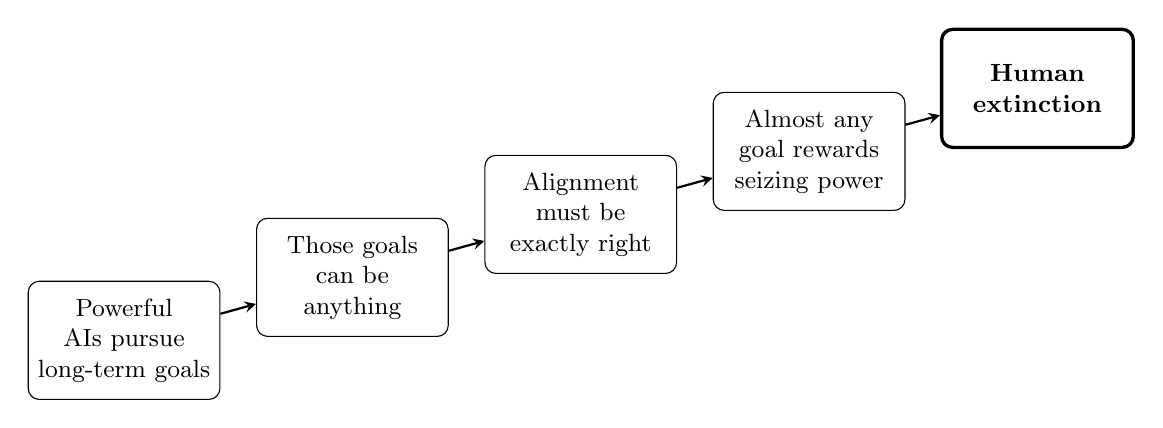
\begin{tikzpicture}[box/.style={draw, rounded corners, align=center, text width=2.2cm, minimum height=1.5cm, font=\small}, >=stealth]
\node[box] (a) at (0,0) {Powerful AIs pursue long-term goals};
\onslide<2->{\node[box] (b) at (2.9,0.8) {Those goals can be anything};}
\onslide<3->{\node[box] (c) at (5.8,1.6) {Alignment must be exactly right};}
\onslide<4->{\node[box] (d) at (8.7,2.4) {Almost any goal rewards seizing power};}
\onslide<5->{\node[box, very thick] (e) at (11.6,3.2) {\textbf{Human extinction}};}
\onslide<2->{\draw[->, thick] (a) -- (b);}
\onslide<3->{\draw[->, thick] (b) -- (c);}
\onslide<4->{\draw[->, thick] (c) -- (d);}
\onslide<5->{\draw[->, thick] (d) -- (e);}
\end{tikzpicture}
\source{yudkowsky2025}
\end{frame}

\begin{frame}{If We Solve Alignment: Extreme Concentration of Power}
\centering
\begin{tikzpicture}[>=stealth]
\node (h) at (0,2.6) {\Huge\faUser};
\foreach \x in {-4,-3,...,4} {
  \node (r\x) at (\x*0.9,0) {\LARGE\faRobot};
  \draw[->, gray] (h) -- (r\x);
}
\end{tikzpicture}

\vspace{1.2em}
Whoever controls the first superintelligence no longer needs anyone else.
\end{frame}

\begin{frame}{RSI and the Race With China}
\begin{columns}[t]
\column{0.5\textwidth}
\centering
\textbf{Independent progress}

\vspace{0.5em}
\begin{tikzpicture}
\node[anchor=south west, inner sep=0] (img) at (0,0) {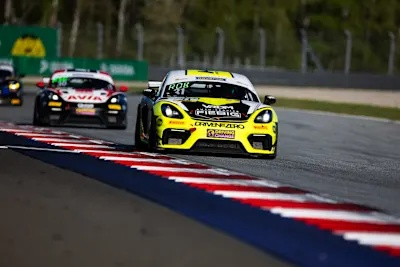
\includegraphics[height=3.9cm]{race_cars}};
\begin{scope}[x={(img.south east)}, y={(img.north west)}]
\coordinate (cn) at (0.16,0.84);
\coordinate (us) at (0.6,0.88);
\end{scope}
\node at (cn) {\worldflag[width=0.75cm]{CN}};
\node at (us) {\worldflag[width=0.75cm]{US}};
\end{tikzpicture}

\vspace{0.5em}
{\small If the US slows down, China simply overtakes\\and reaches RSI first}
\column{0.5\textwidth}
\centering
\textbf{Catch-up growth}

\vspace{0.5em}
\begin{tikzpicture}
\node[anchor=south west, inner sep=0] (img) at (0,0) {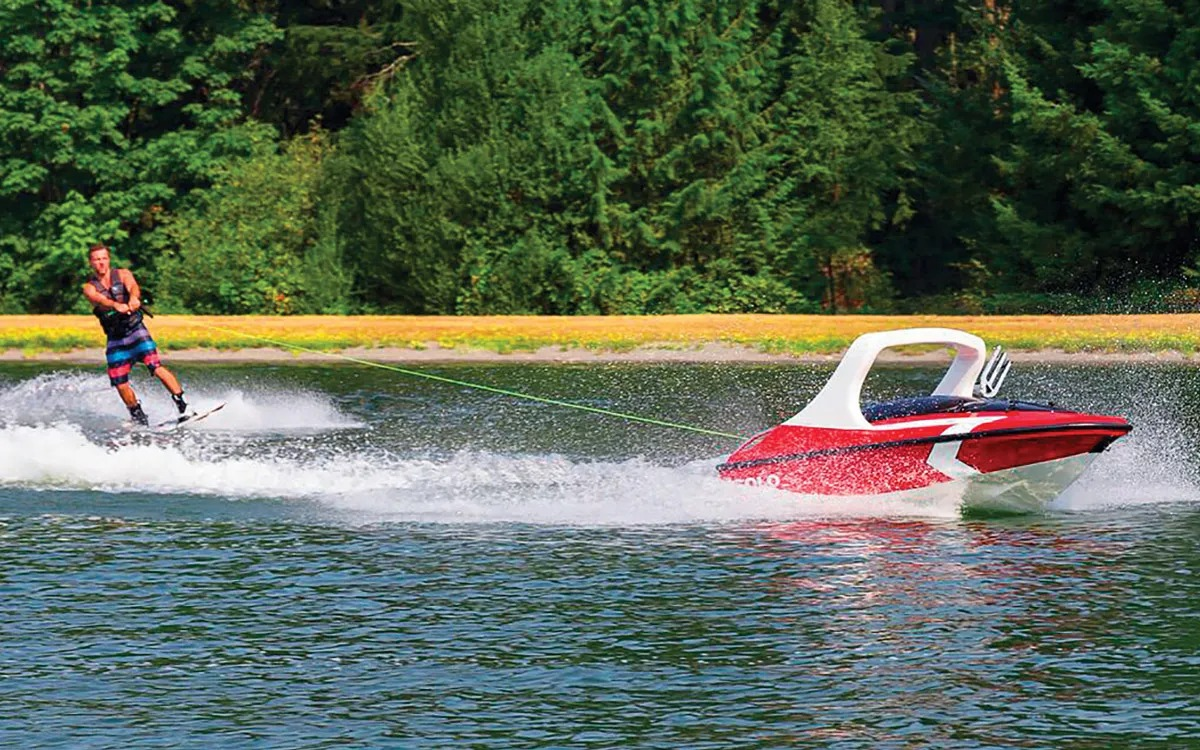
\includegraphics[height=3.9cm]{race_waterski}};
\begin{scope}[x={(img.south east)}, y={(img.north west)}]
\coordinate (cn) at (0.1,0.8);
\coordinate (us) at (0.78,0.7);
\end{scope}
\node at (cn) {\worldflag[width=0.75cm]{CN}};
\node at (us) {\worldflag[width=0.75cm]{US}};
\end{tikzpicture}

\vspace{0.5em}
{\small China is pulled along by distillation and leaked algorithms: slowing down and securing secrets slows both}
\end{columns}
\source{patel2026a}
\end{frame}

\begin{frame}{How Far Ahead Is the US Really?}
\begin{columns}[t]
\column{0.48\textwidth}
\textbf{Hacktron $\to$ OpenAI}
\begin{itemize}
\item An AI security startup, using Claude
\item Within a couple of days: employee accounts and the internal codebase
\item Opened a harmless pull request as proof
\end{itemize}
\column{0.48\textwidth}
\textbf{Cathedral $\to$ Anthropic}
\begin{itemize}
\item Another AI security startup
\item In under 12 hours: internal business systems
\item Including Slack discussions about advanced models, by its own account
\end{itemize}
\end{columns}
\vspace{0.6em}
\pause
\centering
{\large ``In reality, we're 12 hours ahead of China.''}

{\small Dwarkesh Patel}
\source{uko2026,washingtonpost2026,patel2026a}
\end{frame}
